\section{Variational Quantum State Eigensolver (VQSE)} \label{sec:vqse_deep_dive}

TQFI requires a subroutine that extracts the dominant spectral components of the encoded state. We use the Variational Quantum State Eigensolver (VQSE), which performs a task analogous to principal-component extraction while requiring only one $n$-qubit copy of the input state per circuit execution~\cite{cerezo2022vqse}. Our contribution is an independent implementation and benchmark of the protocol. In particular, we implemented the dynamically adjusted auxiliary Hamiltonian described in Section~\ref{sec:vqse_adaptive_cost}, which is designed to mitigate trainability problems such as barren plateaus and local minima. We also investigated two forms of geometry-aware optimization: SR, illustrated in a pure-state neural-quantum-state benchmark and additionally tested as a surrogate on selected small VQSE instances; and a damped Bures natural gradient for adaptive mixed-state VQSE. To the best of our knowledge, this is the first reported independent VQSE implementation to combine the adaptive Hamiltonian with stochastic reconfiguration.


VQSE variationally estimates the $m$ largest eigenvalues $\{\lambda_i\}_{i=1}^m$ and produces a circuit that prepares approximations to their eigenvectors $\{|\lambda_i\rangle\}_{i=1}^m$ for an unknown $n$-qubit density matrix $\rho$~\cite{cerezo2022vqse}. In contrast, VQE targets the ground state of a known Hamiltonian. Figure~\ref{fig:vqse_from_paper} summarizes the VQSE training and readout workflow.

\begin{figure}[htb!]
    \centering
    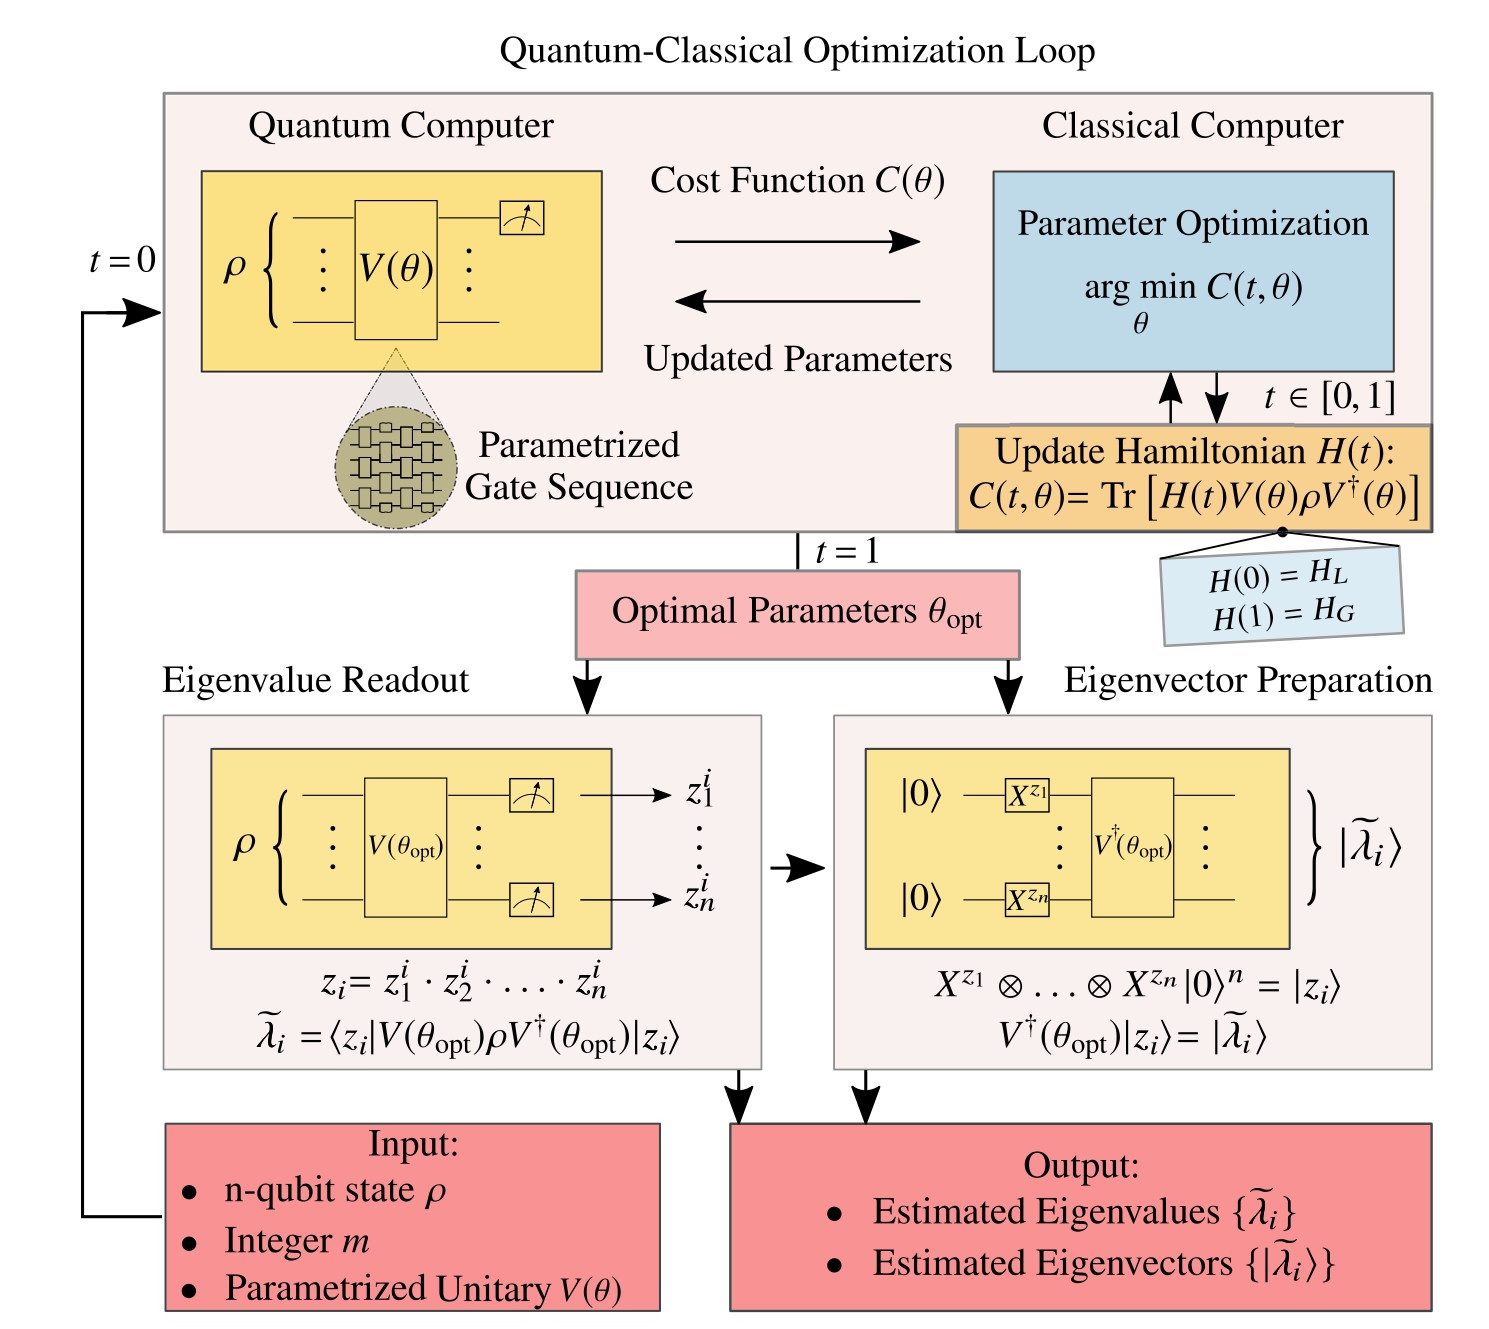
\includegraphics[width=\textwidth]{figures/asi_report/VQSE_frompaper.jpg}
    \caption{VQSE workflow, adapted from~\cite{cerezo2022vqse}. The inputs are an $n$-qubit state $\rho$, the number $m$ of dominant eigenpairs sought, and a parameterized circuit $V(\boldsymbol{\beta})$. In the upper quantum--classical loop, the circuit prepares $\widetilde{\rho}=V(\boldsymbol{\beta})\rho V^\dagger(\boldsymbol{\beta})$; computational-basis measurements supply the cost $C(t,\boldsymbol{\beta})=\operatorname{Tr}[H_{\mathrm{cost}}(t)\widetilde{\rho}]$, and a classical optimizer updates $\boldsymbol{\beta}$ while the auxiliary cost Hamiltonian is adapted. After training, the lower-left circuit measures $\widetilde{\rho}$ at $\boldsymbol{\beta}_{\mathrm{opt}}$: the frequencies of the selected bitstrings $z_i$ estimate the $m$ largest eigenvalues $\widetilde{\lambda}_i$. In the lower-right circuit, preparing $|z_i\rangle$ and applying $V^\dagger(\boldsymbol{\beta}_{\mathrm{opt}})$ gives the corresponding approximate eigenvector $|\widetilde{\lambda}_i\rangle$. The source figure writes $\theta$ for our circuit-parameter vector $\boldsymbol{\beta}$ and $H(t)$ for our $H_{\mathrm{cost}}(t)$; $t\in[0,1]$ denotes normalized optimization progress, not physical evolution time or the sensed parameter $\theta$.}
    \label{fig:vqse_from_paper}
\end{figure}
% ==============================================================================
\subsection{Mathematical Foundation: Diagonalization via Majorization}
% ==============================================================================

VQSE can be understood as sorting eigenvalue weight among
computational-basis outcomes. The unitary $V(\boldsymbol{\beta})$
preserves the eigenvalues of $\rho$, but changes the diagonal
probabilities observed after the basis rotation~\cite{horn_johnson_2012_matrix}. Training seeks to
assign the largest eigenvalues, in order, to selected basis states.
At the ideal optimum, their measurement probabilities equal those
eigenvalues~\cite{cerezo2022vqse}.

Majorization makes this notion of concentration precise: for two lists with the same total, the more concentrated list has a larger or equal sum of its largest $\ell$ entries for every $\ell$.

\begin{definition}[Majorization of the Diagonal]
    Let $d=2^n$, and let the eigenvalues of $\rho$ be ordered as $\lambda_1\geq\lambda_2\geq\cdots\geq\lambda_d\geq0$. After applying $V(\boldsymbol{\beta})$, measurement in the computational basis $\{|z_k\rangle\}$ gives the probabilities
    \begin{equation}
        p_k(\boldsymbol{\beta})
        =\langle z_k|V(\boldsymbol{\beta})\rho
        V^\dagger(\boldsymbol{\beta})|z_k\rangle
    \end{equation}
    Using the spectral decomposition $\rho=\sum_j\lambda_j|\lambda_j\rangle\langle\lambda_j|$, the same probability can be written as
    \begin{equation}
        \begin{aligned}
            p_k(\boldsymbol{\beta}) & = \langle z_k|V(\boldsymbol{\beta}) \left( \sum_{j=1}^d \lambda_j |\lambda_j\rangle\langle\lambda_j| \right) V^\dagger(\boldsymbol{\beta})|z_k\rangle \\
                                    & = \sum_{j=1}^d \lambda_j \langle z_k|V(\boldsymbol{\beta})|\lambda_j\rangle \langle\lambda_j|V^\dagger(\boldsymbol{\beta})|z_k\rangle                 \\
                                    & = \sum_{j=1}^d \lambda_j \left| \langle z_k|V(\boldsymbol{\beta})|\lambda_j\rangle \right|^2
        \end{aligned}
        \label{eq:vqse_probability_mixing}
    \end{equation}


    Thus, the basis change redistributes the eigenvalue weights among the measurement outcomes. The coefficients in this sum are non-negative, and each row and column of the coefficient matrix sums to one.
    If $\mathbf{p}^{\downarrow}$ denotes these probabilities sorted in non-increasing order, the Schur--Horn theorem gives
    \begin{equation}
        \sum_{k=1}^{\ell}p_k^{\downarrow}(\boldsymbol{\beta})
        \leq \sum_{k=1}^{\ell}\lambda_k,
        \qquad \ell=1,\ldots,d-1,
        \qquad
        \sum_{k=1}^{d}p_k(\boldsymbol{\beta})=\sum_{k=1}^{d}\lambda_k=1
        \label{eq:vqse_majorization}
    \end{equation}
    This relation is written $\boldsymbol{\lambda}\succ\mathbf{p}(\boldsymbol{\beta})$. In simple terms, the diagonal probabilities in an arbitrary basis cannot be more concentrated than the eigenvalues. When $V$ rotates the eigenbasis of $\rho$ onto the computational basis, the two lists agree up to a permutation.
\end{definition}

\begin{theorem}[VQSE Cost Function Minimization]
    Let $\rho$ have eigenvalues $\lambda_1\geq\cdots\geq\lambda_d$, as above. Choose a diagonal auxiliary Hamiltonian whose computational-basis states $|z_k\rangle$ are listed in order of nondecreasing energy:
    \begin{equation}
        H_{\mathrm{VQSE}}=\sum_{k=1}^{d}E_k|z_k\rangle\langle z_k|,
        \qquad 0\leq E_1\leq E_2\leq\cdots\leq E_d
    \end{equation}
    For any unitary $V(\boldsymbol{\beta})$, the expectation of this auxiliary Hamiltonian on the transformed state is
    \begin{equation}
        C(\boldsymbol{\beta})
        =\operatorname{Tr}\!\left[H_{\mathrm{VQSE}}
            V(\boldsymbol{\beta})\rho V^\dagger(\boldsymbol{\beta})\right]
        =\sum_{k=1}^{d}E_kp_k(\boldsymbol{\beta})
        \label{eq:vqse_cost_dot_product}
    \end{equation}
    Because the eigenvalue list majorizes the diagonal probability list, the cost obeys
    \begin{equation}
        C(\boldsymbol{\beta})\geq\sum_{k=1}^{d}E_k\lambda_k
        \label{eq:vqse_cost_lower_bound}
    \end{equation}
    The bound is attainable over unrestricted unitaries: a unitary that maps an eigenbasis of $\rho$ to the computational basis in this energy order makes $p_k=\lambda_k$ for every $k$.
\end{theorem}

\begin{remark}[Implication for VQSE]
    The theorem identifies the ideal target for training. If the ansatz can represent the required basis change and optimization finds it, the largest eigenvalues are assigned to the lowest-energy basis states. For the resolved components, one may then choose eigenvectors such that
    \begin{equation}
        V(\boldsymbol{\beta}_{\mathrm{opt}})|\lambda_k\rangle
        =e^{i\phi_k}|z_k\rangle
        \label{eq:vqse_eigenvector_mapping}
    \end{equation}
    Their computational-basis probabilities equal $\lambda_k$, and applying $V^\dagger(\boldsymbol{\beta}_{\mathrm{opt}})$ to $|z_k\rangle$ prepares the corresponding eigenvector up to phase. If the ansatz or optimization falls short of this ideal, VQSE may yield only approximate eigenvalues and eigenvectors; degenerate eigenvalues determine an eigenspace rather than a unique eigenvector basis.
\end{remark}

\begin{remark}[Why the cost sorts the probabilities]
    Consider two basis states with $E_i<E_j$ but $p_i<p_j$. Exchanging their probabilities would lower the cost by $(E_j-E_i)(p_j-p_i)>0$. Thus, minimizing the cost favors larger probabilities at lower energies. This exchange explains the sorting intuition; majorization gives the global lower bound in Eq.~\eqref{eq:vqse_cost_lower_bound}.
\end{remark}

\begin{remark}[How to interpret $H_{\mathrm{VQSE}}$]
    The auxiliary Hamiltonian is a scoring observable chosen by the algorithm; it is not the physical Hamiltonian that produced $\rho$. To extract the $m$ dominant components, its $m$ lowest levels must be non-degenerate so that they give those components distinct labels. The remaining levels may be degenerate because their individual eigenvectors are not needed.
\end{remark}

Operationally, Eq.~\eqref{eq:vqse_cost_dot_product} requires only the measurement probabilities of the transformed state and the known weights $E_k$. VQSE therefore avoids full tomography and does not need to measure every off-diagonal element of $V\rho V^\dagger$.

% ==============================================================================
\subsection{Ansatz Execution and Readout Subroutines}
% ==============================================================================

Once the hybrid quantum--classical loop converges to the parameter set $\boldsymbol{\beta}_{\text{opt}}$, the $m$ dominant eigenvalues and eigenvectors are retrieved as follows:
\begin{enumerate}
    \item \textbf{Eigenvalue readout.} Prepare $V(\boldsymbol{\beta}_{\text{opt}})\rho V^\dagger(\boldsymbol{\beta}_{\text{opt}})$ and sample it in the computational basis for $N_{\text{runs}}$ shots. The estimated eigenvalue associated with bitstring $z_i\in\{0,1\}^n$ is its relative frequency,
          \begin{equation}
              \tilde{\lambda}_i^{\mathrm{est}}=\frac{f_i}{N_{\text{runs}}}
          \end{equation}
    \item \textbf{Eigenvector preparation on demand.} Given the computational-basis state $|z_i\rangle=X^{z_{i,1}}\otimes\dots\otimes X^{z_{i,n}}|0\rangle^{\otimes n}$, the corresponding approximate eigenvector is prepared as
          \begin{equation}
              |\tilde{\lambda}_i\rangle=V^\dagger(\boldsymbol{\beta}_{\text{opt}})|z_i\rangle
          \end{equation}
\end{enumerate}

\begin{algorithm}[H]
    \caption{VQSE Principal Component Extraction}
    \label{alg:vqse}
    \begin{algorithmic}[1]
        \Require Input state $\rho$, truncation rank $m$, parameterized ansatz $V(\boldsymbol{\beta})$, and $H_{\mathrm{VQSE}}$ with $m$ non-degenerate lowest levels.
        \While{not converged}
        \State Prepare $\rho$, apply $V(\boldsymbol{\beta})$, and measure $C(\boldsymbol{\beta})$.
        \State Estimate $\nabla_{\boldsymbol{\beta}}C$ and update $\boldsymbol{\beta}$ with the selected classical optimizer.
        \EndWhile
        \State Sample $V(\boldsymbol{\beta}_{\mathrm{opt}})\rho V^\dagger(\boldsymbol{\beta}_{\mathrm{opt}})$ in the computational basis.
        \State Estimate the $m$ dominant eigenvalues from the most frequent bitstrings and prepare their eigenvectors with $V^\dagger(\boldsymbol{\beta}_{\mathrm{opt}})$.
    \end{algorithmic}
\end{algorithm}

To separate ansatz and optimization error from the unavoidable error caused by rank truncation, Figure~\ref{fig:vqse_infidelity_layers} compares the VQSE reconstruction with direct numerical truncation. Increasing the ansatz depth generally brings the variational reconstruction closer to the numerical rank-$m$ reference, although the convergence is not strictly monotonic. This expressivity--trainability trade-off motivates the adaptive cost introduced next.

\begin{figure}[htb!]
    \centering
    
\includegraphics[width=0.8\textwidth]{asi_report/VQSE_plot.png}
    \caption{VQSE reconstruction infidelity as a function of ansatz depth for an $n=3$ reduced state obtained from an $N=5$ qubit TFIM simulation, with $J=1$, $h_x=0.5$, physical evolution time $t_{\mathrm{evol}}=1$, truncation rank $m=3$, and state purity $0.896$. The blue curve shows $1-F$ between the input state and its VQSE-derived rank-$m$ reconstruction; the maximum iteration count is $50$ times the number of ansatz layers. The dashed horizontal line is the infidelity obtained by direct numerical rank-$m$ truncation and therefore isolates the truncation floor. The vertical axis is logarithmic and inverted, so points higher in the panel have lower infidelity.}
    \label{fig:vqse_infidelity_layers}
\end{figure}

% ==============================================================================

\subsection{Adaptive Cost Function}\label{sec:vqse_adaptive_cost}

The minimization theorem above applies to any fixed diagonal scoring Hamiltonian. In our implementation, we allow this Hamiltonian to change between optimization stages, combining an initially trainable objective with one that distinguishes the dominant spectral components. At each fixed value of the schedule parameter $t$, $H_{\mathrm{cost}}(t)$ remains a diagonal scoring observable and defines the instantaneous VQSE cost.

A shallow variational circuit may not be expressive enough to represent the required eigenbasis transformation, whereas a deep circuit can be difficult to optimize. In particular, barren plateaus are regions where cost gradients become exponentially small with system size for certain ansatzes and objectives. The choice of auxiliary Hamiltonian therefore creates a trade-off between trainability and the structure of the optimization landscape~\cite{cerezo2022vqse}. We implemented and tested the adaptive-cost strategy proposed for VQSE to address this trade-off.

\begin{itemize}

    \item \textbf{Fixed local Hamiltonian.} A choice such as $H_L=\mathbb{I}-\sum_j r_jZ_j$, with coefficients selected so that its $m$ lowest levels are non-degenerate, defines a local cost that can avoid barren plateaus for shallow ansatzes. Its smaller degeneracy restricts the solution space, and the landscape may still contain suboptimal local minima.
    \item \textbf{Fixed global Hamiltonian.} The choice
          \begin{equation}
              H_G=\mathbb{I}-\sum_{i=1}^m q_i|z_i\rangle\langle z_i|,
              \qquad 1\geq q_1>q_2>\dots>q_m>0
              \label{eq:vqse_global_hamiltonian}
          \end{equation}
          has $m$ non-degenerate low-energy levels and a $(2^n-m)$-fold degenerate complementary subspace. This enlarges the solution space, but a global cost can exhibit exponentially vanishing gradients for random hardware-efficient ansatzes.
\end{itemize}

Following~\cite{cerezo2022vqse}, we consider a time-dependent schedule that interpolates between these two costs:
\begin{equation}
    H_{\mathrm{cost}}(t)=[1-f(t)]H_L+f(t)H_G(t),
    \qquad f(0)=0,\quad f(1)=1
    \label{eq:adaptive_hamiltonian}
\end{equation}
where $t=k/N_{\max}$ represents normalized optimization progress. The schedule $f(t)$ should increase gradually so that the early optimization is governed mainly by the trainable local cost.


As outlined in Algorithm~\ref{alg:adaptive_vqse}, the global component
\begin{equation}
    H_G(t)=\mathbb{I}-\sum_{i=1}^m q_i|z_i(t)\rangle\langle z_i(t)|
\end{equation}
is periodically updated using the dominant bitstrings sampled from $V(\boldsymbol{\beta})\rho V^\dagger(\boldsymbol{\beta})$. The operator remains a global cost. Here ``adaptive'' means that the selected basis states change during training. The construction and its trainability motivation follow Ref.~\cite{cerezo2022vqse}; its practical performance still depends on the chosen ansatz and noise model and is therefore assessed empirically here. Finite-shot effects are discussed in Appendix~\ref{appendix:finite_shot_sampling}.

\begin{algorithm}[H]
    \caption{Adaptive VQSE Optimization Schedule}
    \label{alg:adaptive_vqse}
    \begin{algorithmic}[1]
        \Require Input state $\rho$, rank $m$, ansatz $V(\boldsymbol{\beta})$, maximum iteration count $N_{\max}$, update interval $s$, schedule $f$, local $H_L$, weights $\{q_i\}_{i=1}^m$.
        \State Initialize $\boldsymbol{\beta}$ randomly and set $H_{\mathrm{cost}}(0)\leftarrow H_L$.
        \For{$k=1,2,\ldots,N_{\max}$}
        \State Set $t\leftarrow k/N_{\max}$.
        \If{$k=1$ or $k\bmod s=0$}
        \State Measure $V(\boldsymbol{\beta})\rho V^\dagger(\boldsymbol{\beta})$ in the computational basis.
        \State Identify $m$ most frequent bitstrings $Z(t) = \{z_1(t), \dots, z_m(t)\}$.
        \State Update $H_G(t)\leftarrow\mathbb{I}-\sum_{i=1}^m q_i|z_i(t)\rangle\langle z_i(t)|$.
        \EndIf
        \State Update $H_{\mathrm{cost}}(t)\leftarrow[1-f(t)]H_L+f(t)H_G(t)$.
        \State Execute a classical optimization step: $\boldsymbol{\beta} \leftarrow \text{Optimizer}(\boldsymbol{\beta}, \nabla_{\boldsymbol{\beta}} C(t, \boldsymbol{\beta}))$.
        \EndFor
        \State \textbf{Return:} $\boldsymbol{\beta}_{\text{opt}} \leftarrow \boldsymbol{\beta}$.
    \end{algorithmic}
\end{algorithm}
Figure~\ref{fig:vqse_adaptive_cost} shows the evolution of the adaptive cost in one of our optimization runs.

\begin{figure}[htb!]
    \centering
    
\includegraphics[width=0.8\textwidth]{misc/VQSE_adaptive_training.png}
    \caption{Adaptive VQSE training for a two-qubit mixed state with spectrum $(0.40,0.28,0.20,0.12)$, a rank-$3$ target, two Strongly Entangling Layers, $50$ outer iterations, and five BFGS~\cite{bfgs_alg} steps per iteration. The upper panel shows the adaptive objective together with the instantaneous local and global objectives. The lower panel shows the local and global weights for the quadratic schedule $H_{\mathrm{cost}}(t)=(1-t^2)H_L+t^2H_G(t)$. Vertical white lines mark global-target refreshes every five iterations. The adaptive objective decreases from $0.726$ to $0.409$, and the final $\ell_2$ error of the three leading eigenvalues is $1.741\times10^{-2}$.}
    \label{fig:vqse_adaptive_cost}
\end{figure}

\subsection{Geometry-Aware Optimization of VQSE}\label{sec:vqse_qng_optimization}

Quantum natural-gradient descent (QNG) accounts for the local geometry of the ansatz-state family instead of treating the circuit parameters as Euclidean coordinates. The ansatz QFIM and the general QNG update are defined in Eqs.~\eqref{eq:ansatz_qfim} and~\eqref{eq:qng_update}.

\noindent\faLightbulb\hspace{5pt}\textbf{In simple terms}: the ansatz QFIM preconditions the standard gradient. Omitting the learning rate and regularization, the geometry-aware descent direction for VQSE is
$-[F^{\mathrm{ans}}]^{-1}\nabla_{\boldsymbol{\beta}}C$.

For VQSE, the trainable variables are the circuit parameters $\boldsymbol{\beta}$ and the adaptive objective is
\begin{equation}
    C(t,\boldsymbol{\beta})
    =\operatorname{Tr}\!\left[
        H_{\mathrm{cost}}(t)
        V(\boldsymbol{\beta})\rho V^\dagger(\boldsymbol{\beta})
        \right]
    \label{eq:vqse_adaptive_objective}
\end{equation}
A geometry-aware optimizer preconditions $\nabla_{\boldsymbol{\beta}}C$ using a metric on this circuit-parameter space. This ansatz geometry concerns the adjustable training parameters and must be distinguished from the QFI associated with the unknown physical parameter $h_x$.

This gives the procedure an \enquote{inception-like} structure: the QFIM of the ansatz state helps to train an algorithm that is itself used to estimate QFI \inceptiontop[0.2]~\cite{nolan2010inception}.

The related pure-state construction can be illustrated particularly clearly using a neural quantum state. The following infobox is an independent optimizer benchmark, not a mixed-state VQSE result.

\begin{infobox}[infobox:sr_nqs_example]{Stochastic Reconfiguration for a Neural Quantum State}
    Stochastic reconfiguration (SR) provides a sampled form of natural-gradient optimization for a neural quantum state~\cite{Park2020_geometry_learning_neural_quantum_states}.  For a wavefunction $\Psi_{\boldsymbol{\vartheta}}(\boldsymbol{\sigma})$, define the logarithmic derivatives and their covariance matrix by
    \begin{equation}
        \mathcal{O}_i(\boldsymbol{\sigma})
        =\partial_{\vartheta_i}\log\Psi_{\boldsymbol{\vartheta}}(\boldsymbol{\sigma})
        \qquad
        S_{ij}
        =\operatorname{Re}\!\left[
            \langle\mathcal{O}_i^*\mathcal{O}_j\rangle
            -\langle\mathcal{O}_i^*\rangle\langle\mathcal{O}_j\rangle
            \right]
        \label{eq:sr_covariance_metric}
    \end{equation}
    For a normalized pure wavefunction, $S$ represents the Fubini--Study metric up to the chosen normalization convention.  The regularized SR update is
    \begin{equation}
        \boldsymbol{\vartheta}_{k+1}
        =\boldsymbol{\vartheta}_k
        -\eta\left(S+\lambda\mathbb{I}\right)^{-1}
        \nabla_{\boldsymbol{\vartheta}}E
        \qquad
        \lambda\geq0
        \label{eq:sr_parameter_update}
    \end{equation}

    We tested this principle with a real, positive restricted Boltzmann machine (RBM) wavefunction for the TFIM. The implementation uses $N$ visible units for the physical spins and $M$ hidden units. It evaluates the logarithmic derivatives in Eq.~\eqref{eq:sr_covariance_metric}, estimates $S$ and the energy gradient from variational Monte Carlo samples, adds the diagonal regularization $\lambda\mathbb{I}$, and solves the resulting linear system. Figure~\ref{fig:sgd_vs_ng} compares SR with ordinary stochastic gradient descent in this tractable pure-state example.

    \begin{figure}[H]
        \centering
        
\includegraphics[width=\linewidth]{misc/sgd_vs_sr_comparison-set2-palette.png}
        \caption{Energy minimization for a periodic $N=8$ TFIM at $g=h_x/J=1$ using a real, positive RBM neural quantum state with $M=8$ hidden units ($M/N=1$)~\cite{carleo2017nqs}. Both optimizers use $80$ steps, $300$ Monte Carlo samples per step, a learning rate of $0.05$, a gradient-norm clipping threshold of $1$, and random seed $42$. SR uses the diagonal regularization $\lambda=10^{-4}$. The left panel shows the estimated energy together with the exact ground-state energy; the right panel shows the corresponding absolute error on a logarithmic scale. In this run, SR converges to a lower final error than ordinary stochastic gradient descent.}
        \label{fig:sgd_vs_ng}
    \end{figure}

\end{infobox}

On selected small VQSE instances, we also tested the SR principle as a surrogate preconditioner. Applying it to VQSE requires care because $V(\boldsymbol{\beta})\rho V^\dagger(\boldsymbol{\beta})$ remains mixed when the input $\rho$ is mixed. The intrinsic metric is then the mixed-state ansatz QFIM; a pure-state Fubini--Study or SR metric is only a surrogate unless a suitable purification or mixed-state estimator is used. Moreover, a full metric for $N_{\mathrm{par}}$ circuit parameters contains $\mathcal{O}(N_{\mathrm{par}}^2)$ elements, and solving the regularized update adds a substantial classical cost~\cite{kolotouros2024RNG,gacon2021_perturbation_stochastic_qfi}.

For the mixed-state comparison in Figure~\ref{fig:vqse_optimizer_comparison}, we use the Bures metric of the VQSE ansatz family
$\widetilde{\rho}_{\boldsymbol{\beta}}=V(\boldsymbol{\beta})\rho V^\dagger(\boldsymbol{\beta})$. At regular points,
$g^{\mathrm B}(\boldsymbol{\beta})=F^{\mathrm{ans}}(\boldsymbol{\beta})/4$, by Eq.~\eqref{def:qfim_bures_relation}. The deterministic damped Bures natural-gradient step is
\begin{equation}
    \Delta\boldsymbol{\beta}_k
    =-\eta\left[
        g^{\mathrm B}(\boldsymbol{\beta}_k)+\lambda\mathbb{I}
        \right]^{-1}
    \nabla_{\boldsymbol{\beta}}C(t_k,\boldsymbol{\beta}_k),
    \qquad \lambda>0
    \label{eq:vqse_bures_natural_gradient}
\end{equation}
This is the mixed-state Bures-metric form of the QNG update in Eq.~\eqref{eq:qng_update}; the factor of four relating $g^{\mathrm B}$ and $F^{\mathrm{ans}}$ is absorbed into the learning-rate and damping conventions. The inverse metric suppresses directions that produce a large Bures displacement and gives greater relative weight to directions with smaller metric eigenvalues, while the damping $\lambda$ limits ill-conditioned updates. In this benchmark, that geometric preconditioning is consistent with the smoother late-stage update sequence visible in Figure~\ref{fig:vqse_optimizer_comparison}.

\begin{figure}[htb!]
    \centering
    
\includegraphics[width=\textwidth]{misc/VQSE_optimizer_comparison.png}
    \caption{Comparison of BFGS~\cite{bfgs_alg}, Adam, and Bures natural-gradient optimization for adaptive VQSE. \emph{Top left:} the leading-spectrum error $\lVert\widetilde{\boldsymbol{\lambda}}_{1:3}-\boldsymbol{\lambda}_{1:3}\rVert_2$ relative to the exact eigenvalues, shown on a logarithmic scale. Unlike the adaptive objective, the definition of this diagnostic does not change when the global target is refreshed. \emph{Top right:} the adaptive objective $C(t,\boldsymbol{\beta})=\operatorname{Tr}[H_{\mathrm{cost}}(t)\widetilde{\rho}_{\boldsymbol{\beta}}]$. Because $H_{\mathrm{cost}}(t)$ changes during the local-to-global transition, this panel should not be interpreted by itself as a fixed-loss convergence curve. \emph{Bottom left:} the final three leading eigenvalue estimates and the exact spectrum. \emph{Bottom right:} the Euclidean update norm $\lVert\Delta\boldsymbol{\beta}\rVert_2$ on a logarithmic scale. BFGS shows spikes, while Bures natural gradient shows a smoother sequence of progressively smaller updates after its initial adjustment. The vertical markers in the top-left panel denote refreshes of the global target.}
    \label{fig:vqse_optimizer_comparison}
\end{figure}

% ==============================================================================
\subsection{Comparative Resource Scaling: Why VQSE is Qubit-Frugal}
% ==============================================================================

Compared with the other state-diagonalization and principal-component methods considered here, the principal qubit-count advantage of VQSE is that its optimization cost requires only a \textbf{single copy of $\rho$ ($n$ qubits)} per circuit execution~\cite{cerezo2022vqse}. Optional overlap-based verification can require a second copy. Table~\ref{tab:vqse_comparison} summarizes the comparison.

\begin{table}[H]
    \centering
    \caption{Quantum resources and principal NISQ bottlenecks of the state-spectrum extraction methods considered for an $n$-qubit density matrix $\rho$.}
    \label{tab:vqse_comparison}
    \begin{tabular}{p{2.25cm} p{2.2cm} p{2.6cm} p{5.75cm}}
        \toprule
        \textbf{Algorithm} & \textbf{Qubit Count} & \textbf{Input State}           & \textbf{Primary NISQ Bottlenecks}                                                                               \\
        \midrule
        \textbf{qPCA}      & $n + a$ qubits       & $\rho^{\otimes k}$ copies      & Requires Phase Estimation and matrix exponentiation $e^{-i\rho t}$; prohibitive circuit depth \cite{qpca_2014}. \\
        \textbf{VQSD}      & $2n$ qubits          & $\rho \otimes \rho$ (2 copies) & Requires joint 2-register gates; vulnerable to asymmetric inter-register noise \cite{LaRose2019_vqsd}.          \\
        \textbf{QSVD}      & $n$ to $2n$ qubits   & \makecell{$|\psi_{AB}\rangle$                                                                                                                    \\ (Purification)} & Requires explicit access to a purification, whose preparation is sensitive to uncharacterized noise \cite{Bravo_Prieto_2020_qsvd}. \\
        \textbf{VQSE}      & \textbf{$n$ qubits}  & \textbf{$\rho$ (1 copy)}       & \textbf{Uses a single-copy, majorization-based cost evaluation} \cite{cerezo2022vqse}.                          \\
        \bottomrule
    \end{tabular}
\end{table}

The adaptive cost and geometry-aware optimization studied above provide the dominant eigenvalues and eigenvector-preparation circuits required by the truncated-fidelity bounds. The following section places these VQSE outputs inside the complete VQFIE estimation and optional probe-optimization loop.
